\documentclass[10pt,twocolumn,letterpaper]{article}
\usepackage[T1]{fontenc}
\usepackage[pagenumbers]{cvpr}
\usepackage{graphicx,amsmath,amssymb,booktabs,microtype,balance}
\usepackage[breaklinks,colorlinks,allcolors=black]{hyperref}
\def\confName{CVPR}\def\confYear{2027}
\newcommand{\E}{\mathbb{E}}
\newcommand{\Var}{\operatorname{Var}}
\newcommand{\gfpath}{../../output/gap-first-v01}
\setlength{\textfloatsep}{8pt plus 1pt minus 1pt}
\setlength{\dbltextfloatsep}{8pt plus 1pt minus 1pt}
\title{When Does the Next Interaction Need More Evidence?\\Task-Conditional Risk in Visual Physical Twins}
\author{Experimental addendum to \emph{Seeing Motion Is Not Identifying Mechanics}}
\renewcommand{\dbltopfraction}{.95}
\renewcommand{\topfraction}{.9}
\renewcommand{\textfraction}{.03}
\renewcommand{\floatpagefraction}{.8}
\renewcommand{\dblfloatpagefraction}{.8}
\setcounter{dbltopnumber}{3}
\begin{document}
\twocolumn[{
\renewcommand{\twocolumn}[1][]{#1}
\maketitle
\begin{center}
\includegraphics[width=.98\textwidth]{\gfpath/drop/native-drop-teaser.pdf}
\captionof{figure}{\textbf{An observed drop does not determine the next response.} Two constructed physical explanations share the released ReconPhys appearance and nearly identical passive motion. A reset interaction with the same known body force separates them. Appearance is a released reconstructed asset; mechanics are the declared synthetic hypotheses. The common illustration camera is separate from the frozen cameras used for quantitative image comparison.}
\label{fig:drop-teaser}
\end{center}
}]
\begin{abstract}
Visual agreement and plausible simulation do not establish that an object will respond correctly to a new interaction. This addendum asks a narrower, actionable question: does uncertainty in the physical explanation matter for the next specified task, and should the system proceed, look, or push? We separate three experiments: a native released Gaussian physical model for a drop counterexample, an independently verified compliant-stem reference for evidence selection, and a nonlinear bowl-contact stress test. In the stem study, 96 independent objects are evaluated under three matched task/visibility conditions. Repeating the original interaction requires no additional observation. For a different load location, sparse initial evidence gives 0.939\,mm prediction RMSE; a view-or-proceed policy gives 0.073\,mm when the base is visible, and a probe-or-proceed policy gives 0.119\,mm when it is concealed. Every point baseline receives the same corrective evidence. A strong Gaussian moment-risk baseline performs similarly, so the result establishes task-dependent ambiguity and correction rather than a new universally superior acquisition algorithm. The bowl stress test exposes a distinct failure: after calibration, a coarse model predicts 1.9\% failure risk but fails in 43.8\% of finer-reference cases. A predeclared resolution mixture repairs this constructed mismatch because it includes the finer model. Predictions and risk scores are frozen before held-out outcomes are evaluated.
\end{abstract}

\section{The gap and the question}
A physical reconstruction has at least three distinct obligations: explain the observed images, reproduce observed motion, and predict a changed interaction. Success at the first two does not imply the third. Conversely, uncertainty about a material need not prevent a reliable task prediction. A robot should therefore judge uncertainty through the outcome it needs, not only through the width of a material interval.

Recent systems already connect Gaussian appearance and simulation, including PhysTwin~\cite{phystwin} and ReconPhys~\cite{reconphys}. GaussianBench explicitly evaluates physical fidelity and counterfactual behavior~\cite{gaussianbench}. We do not claim to be the first to identify this distinction. Our experiment concerns the \emph{pre-outcome decision}: whether a named model's next prediction is risky, and whether a new observation reduces that risk.

This is a scoped addition to the existing joint material--interaction study. The earlier spatial Gaussian fields, conditional analytical force marginalization, continuous inference, rendering experiments and contact benchmarks remain separate evidence. The stem is a two-coordinate mechanical reference, not a claim to have trained a new video model. The drop uses released Gaussian appearance and mechanics; the bowl uses nonlinear mechanics with approximate finite-hypothesis inference. These experiments are not presented as one end-to-end raw-video pipeline.

\section{Predict a model's failure before the outcome}
Let $D$ denote available observations, $\theta$ a physical explanation, $a_\star$ a specified future interaction and $q(\theta,a_\star)$ its physical response. For a frozen point prediction $\hat q_j(D,a_\star)$ and application tolerance $\delta$, define
\begin{equation}
 r_j(D,a_\star)=\Pr\!\left(\ell(q(\theta,a_\star),\hat q_j)>\delta\mid D\right).
 \label{eq:risk}
\end{equation}
This is a risk score for a \emph{named prediction}. Posterior variance alone is not the probability that an arbitrary model is wrong. The point model can be a posterior mean, maximum-likelihood estimate or an external frozen predictor. A maximum-likelihood point does not itself supply uncertainty; when we score that point, the uncertainty comes from the reference posterior.

For a possible measurement action $a$, integrate over its unknown observation $y_a$ before choosing:
\begin{equation}
 J(a)=\E_{y_a\mid D,a}[r_j(D\cup\{y_a\},a_\star)]+c(a).
 \label{eq:design}
\end{equation}
The finite action set also contains \emph{proceed}, with $J=r_j(D,a_\star)$ and zero measurement cost. The future interaction specification is known during planning; its realized response and hidden physical parameters are withheld. Sensor noise enters the measurement likelihood. The target error in Eq.~\ref{eq:risk} concerns the physical response, without adding artificial target sensor noise.

Our stem planner uses the posterior-mean predictor. This mean minimizes squared error, not threshold loss in general; Eq.~\ref{eq:design} therefore evaluates its actual threshold risk rather than claiming to optimize the point estimate under every loss. Two worlds with the same observations and the same frozen prediction receive the same pre-action risk. The method recognizes a risky task, not which indistinguishable hidden world is true.

\section{Drop: native-model ambiguity}
We replay the released ReconPhys~\cite{reconphys} solver and Gaussian renderer on the first three lexicographically ordered released assets (pastry, shell, bottle), with 2,048 control anchors, 30 frames and four native cameras. Worlds A and B use $(m,k,d)=(1,300,1)$ and $(2,600,2)$, respectively, with identical geometry, initial state and friction. Scaling mass, spring stiffness and damping together preserves gravity-driven motion in this native hard-floor model. The largest numerical state discrepancy is $1.79\times10^{-7}$ scene units; passive RGB agreement is 94.60--100.08\,dB. Holding mass fixed while changing stiffness instead produces trajectory coordinate RMS differences of 0.0301--0.0424. A known uniform upward body force of 20 units \emph{per anchor}, applied during frames 12--17, breaks the scale ambiguity (Table~\ref{tab:drop}). These are native normalized scene units and spring coefficients, not calibrated SI material parameters or a localized contact poke.

Figure~\ref{fig:drop-teaser} shows the first predeclared asset; the released comparison video and full contact sheet include all three.

\begin{table}[t]
\centering\small\setlength{\tabcolsep}{3pt}
\caption{Native drop counterexample. Gap and errors are scalar-coordinate RMS of the 3D centroid over frames 18--24, in normalized scene units. MAP is updated using the same corrective observation.}
\label{tab:drop}
\begin{tabular}{lrrr}\toprule
Asset & Passive PSNR & Force gap & MAP before $\to$ after\\\midrule
Pastry & 97.60 & 0.188 & $0.0938\to0$\\
Shell & 100.08 & 0.121 & $0.0604\to0$\\
Bottle & 94.60 & 0.219 & $0.1096\to0$\\\bottomrule
\end{tabular}
\end{table}
A separate horizontal calibration force supplies a camera-0 foreground-centroid displacement, with total Gaussian measurement noise $\sigma=0.002$ in normalized image coordinates. With a balanced two-world prior, 100 noise repeats per world and asset select the correct world in all 600 trials; prior failure risk is 0.5 and no corrected prediction exceeds the declared 0.01 coordinate-RMS tolerance. These are three geometries with repeated noise, not 600 independent objects. The same-evidence MAP baseline attains identical point accuracy. This is a finite-candidate identification control, not a demonstration of continuous calibration or a superior acquisition policy.

\paragraph{Whose prediction is at risk?}
In a separately frozen posthoc extension, the unchanged pretrained ReconPhys predictor receives each constructed passive-A movie before its inferred parameters are replayed under the held force. Mean response errors are 0.2245, 0.1666 and 0.2635; both candidate worlds exceed tolerance, so the reference posterior assigns this named prediction risk one. The native predictor remains fixed after calibration; the corrected MAP is a separate refit, not a retrained network. On constructed passive sequences, its view-0 pooled-MSE future-image PSNR is 18.87--21.84\,dB, so model-fit error is distinct from the exact forward ambiguity. Separately, original released-video controls give mean per-frame, four-view future PSNR 18.55/17.74/20.79\,dB for pretrained parameters versus 20.14/21.66/21.43\,dB for released ground-truth parameters under the demo's sampled anchor graph. The imperfect latter replay prevents attributing all discrepancy to the predictor. The extension has no native-success cases and therefore does not establish risk discrimination across the network's operating range. Neither the scale counterexample nor this small extension establishes general end-to-end video identification failure.


\section{Stem: proceed, look, or push}
\begin{figure*}[t]
\centering\includegraphics[width=\textwidth]{\gfpath/stem/stem-mechanical-ambiguity.pdf}
\caption{\textbf{The same initial tip measurement can conceal different mechanics.} A translates mainly through bending; B mainly through its compliant base. Only the original tip displacement is identical. Full geometry is shown here for explanation and would provide additional evidence if visible. The halfway and third-location forces are applied at those locations; they are not measurements of the original tip-loaded shape. All positions use actual mechanical scale.}
\label{fig:stem}
\end{figure*}
\paragraph{A checkable reference.}
An Euler--Bernoulli stem of length $L$ has flexural rigidity $EI$ and a translating, rotation-constrained base with stiffness $k_b$. Under a known point force $F$ at height $a$, displacement at $x$ is
\begin{align}
 u(x;a,F)&=F\left[s+\frac{G(x,a)}{EI}\right],\qquad s=k_b^{-1},\\
 G(x,a)&=\frac{\min(x,a)^2[3\max(x,a)-\min(x,a)]}{6}.
 \label{eq:green}
\end{align}
Writing bending compliance as $b=L^3/(3EI)$, the tip observation is $u(L;L,F)=F(b+s)$. It identifies a sum, not its bending and support contributions.

For specimen A, $(b,s)=(0.4,0.1)$\,m/N; for B, $(0.1,0.4)$\,m/N. A 20\,mN tip force produces 10\,mm in both. A new force at $a=L/2$, measured there, produces 3.00 versus 8.25\,mm, a 2.75-fold difference. A third load at $a=0.75L$ produces 5.375 versus 8.84375\,mm. In contrast, observing the midpoint during the \emph{original tip force} gives 4.50 versus 8.625\,mm. This distinction matters for separating looking from intervening.

\paragraph{What is visible.}
The initial observation is a noisy tip displacement. In the visible-base condition, a simultaneous new view measures the base marker under the same initial force. In the concealed-base condition, the permitted camera menu reveals only another tip measurement; it cannot see the fixture or intermediate stem. This is an explicit access restriction, not a claim that every conceivable view is uninformative. We separately vary the lowest visible marker to show when additional shape information suffices.

\paragraph{Qualified mechanics.}
An independent cubic-Hermite beam assembly checks all three lengths (0.10, 0.12 and 0.15\,m), four compliance corners, five load locations and three discretizations: 180 checks, with maximum nodal discrepancy $1.78\times10^{-10}$\,m. The cross section is $10\times8$\,mm. Worst bending strain is 1.152\% and slope 0.144\,rad. A shear estimate at the shortest probing length contributes at most 0.017\,mm, below the declared 0.15\,mm probe noise. These are linear-beam qualifications, not nonlinear 3D validation.

\paragraph{Inference and data separation.}
The continuous reference prior is independent uniform $b,s\in[0.04,0.48]$\,m/N. Midpoint quadrature uses $129^2$ hypotheses. Gaussian observation noise is 0.10\,mm for initial/view measurements and 0.15\,mm for probing. Probe candidates are $a/L\in\{0.35,0.50,0.65\}$; the withheld task is $a/L=0.75$. Repeated-tip control tasks instead repeat the initial interaction. The tolerance is 0.50\,mm. Look and push costs are 0.015 and 0.040 in the declared failure-probability objective; these are experimental utility choices, not measured robot costs.

The cohort contains 96 independently drawn physical cases with three matched task/access conditions each (288 records, not 288 independent objects). Planning receives only initial measurements, geometry and the task/access condition. Protocol, source, hidden-truth and observation hashes are frozen; a separate process records all predictions and risks before outcomes are evaluated. All policies choosing the same measurement receive exactly the same noisy value. The baseline point estimates are recomputed from that same evidence.

\begin{figure*}[t]
\centering\includegraphics[width=.98\textwidth]{\gfpath/stem/stem-posterior-and-task-risk.pdf}
\caption{\textbf{Parameter ambiguity and task risk are different.} The initial tip measurement leaves a ridge in bending/base compliance. A calibrated push can collapse that ridge. Before probing, repeating the tip load is predictable while a new load is risky. A/B are marked within the continuous-prior posterior. The corrective reading is noiseless and generated from A; the cohort uses noisy measurements. Density colors are normalized separately in the two posterior panels to reveal their support.}
\label{fig:posterior}
\end{figure*}

\paragraph{Numerical reference audit.}
Forty-five truth-free development plans compare quadrature grids through $513^2$ and predictive observation integration through 641 bins. The maximum action-objective change is 0.00125 and all selected actions agree. Integration retains both observation tails. An independently reproduced floating-point endpoint bug in discrete quantiles is corrected in a new helper; historical sources and results are not overwritten. The final policy compares all action objectives directly. A pre-outcome development revision removed a hard stopping gate that could skip a cost-effective view; both versions and the reason are retained.

\section{Stem outcomes and controls}
\begin{table}[t]
\centering\small\setlength{\tabcolsep}{3.5pt}
\caption{Held-out response RMSE (mm), 96 matched cases per column. Lower is better. Accuracy alone omits the cost of acquiring additional evidence.}
\label{tab:stem}
\begin{tabular}{lrrr}\toprule
Policy & Repeat tip & Visible base & Hidden base\\\midrule
Proceed & 0.104 & 0.939 & 0.939\\
Always look & 0.071 & 0.071 & 0.932\\
Always push halfway & 0.105 & 0.097 & 0.097\\
Gaussian moment risk & 0.104 & 0.073 & 0.114\\
Full posterior risk & 0.104 & 0.073 & 0.119\\\bottomrule
\end{tabular}
\end{table}
The uncorrected new-load prediction exceeds tolerance in 52/96 cases (54.17\%). The risk policy has zero observed failures in all three conditions. It proceeds in all 96 repeat-tip cases, chooses a view in 92/96 visible-base cases and a 0.35-height push in 91/96 concealed-base cases. Remaining cases proceed because their task uncertainty is already small under the declared prior.

This is not a universal acquisition win. A cost-aware Gaussian moment approximation also has zero failures and very similar choices. Full posterior minus Gaussian in mean failure-plus-cost is only $-0.000330$, with a 95\% case-bootstrap interval $[-0.000851,0]$ for full posterior minus Gaussian. There is no convincing advantage over that strong simple baseline. Fixed halfway probes achieve lower concealed-base RMSE but spend a measurement on every repeat-tip case and whenever a cheaper view suffices. The full method's lower failure-plus-cost than always probing ($-0.02257$, interval $[-0.02347,-0.02186]$) reflects this declared cost tradeoff.

Posterior intervals and risk are conditional on the specified model and prior. Selected-policy nominal 90\% response coverage is 87.5\%, 89.6\% and 87.5\% across the three conditions. Before correction, mean predicted new-load failure probability is 62.3\%, versus 54.2\% realized failure in this finite cohort. These synthetic results do not establish calibration under unknown tracking errors, nonlinear mechanics or arbitrary real-world material distributions.

\begin{figure}[t]
\centering\includegraphics[width=\columnwidth]{\gfpath/stem/stem-visibility.pdf}
\caption{\textbf{When does looking suffice?} Posterior-predictive risk falls as a camera can measure a marker farther below the tip during the original tip load. This truth-free design sweep fixes the initial observation at 10\,mm; it is not an additional empirical calibration cohort. The dashed line marks 10\% risk for reference, not a hard action-selection gate.}
\end{figure}

\section{Nonlinear bowl contact under position control}
\label{sec:gap-first-bowl}
We test a soft, tapered nonbox solid falling under gravity into a known rigid
hemispherical bowl (radius 90\,mm), followed by a position-controlled interaction.
The model uses compressible Neo--Hookean tetrahedral mechanics, material-surface
quadrature, penalty contact and regularized friction. It is a bounded nonlinear
contact approximation, not the exact Gaussian force-elimination model.
Geometry, density, damping and gravity are known; Young's modulus and a shared
bowl/tool friction coefficient are uncertain.

\begin{table*}[t]
\centering\small
\begin{tabular}{llrrrrr}
\toprule
Reference & Posterior & Initial motion & After motion & Bowl force & Tool force & Brier \\
 & & \multicolumn{2}{c}{MAP RMS (mm)} & \multicolumn{2}{c}{MAP vector RMS (N)} & \\
\midrule
Matched & Coarse only & 7.59 & 0.02 & 0.001 & 0.001 & 0.000 \\
Matched & Resolution mixture & 8.07 & 0.06 & 0.008 & 0.007 & 0.000 \\
Finer reference & Coarse only & 6.98 & 3.09 & 0.335 & 0.335 & 0.412 \\
Finer reference & Resolution mixture & 3.23 & 0.05 & 0.005 & 0.006 & 0.000 \\
\bottomrule
\end{tabular}
\caption{Bowl study, mean over 16 parameter worlds and two noise replicates.
``After'' uses one selected calibration experiment. Finer-reference results are a
space/time-discretization stress; the secondary mixture contains that reference
model by construction. Full clustered intervals, both fixed controls and conditional
motion/force coverage are retained in the report.}
\label{tab:bowl-gap-results}
\end{table*}
\begin{figure*}[t]
\centering
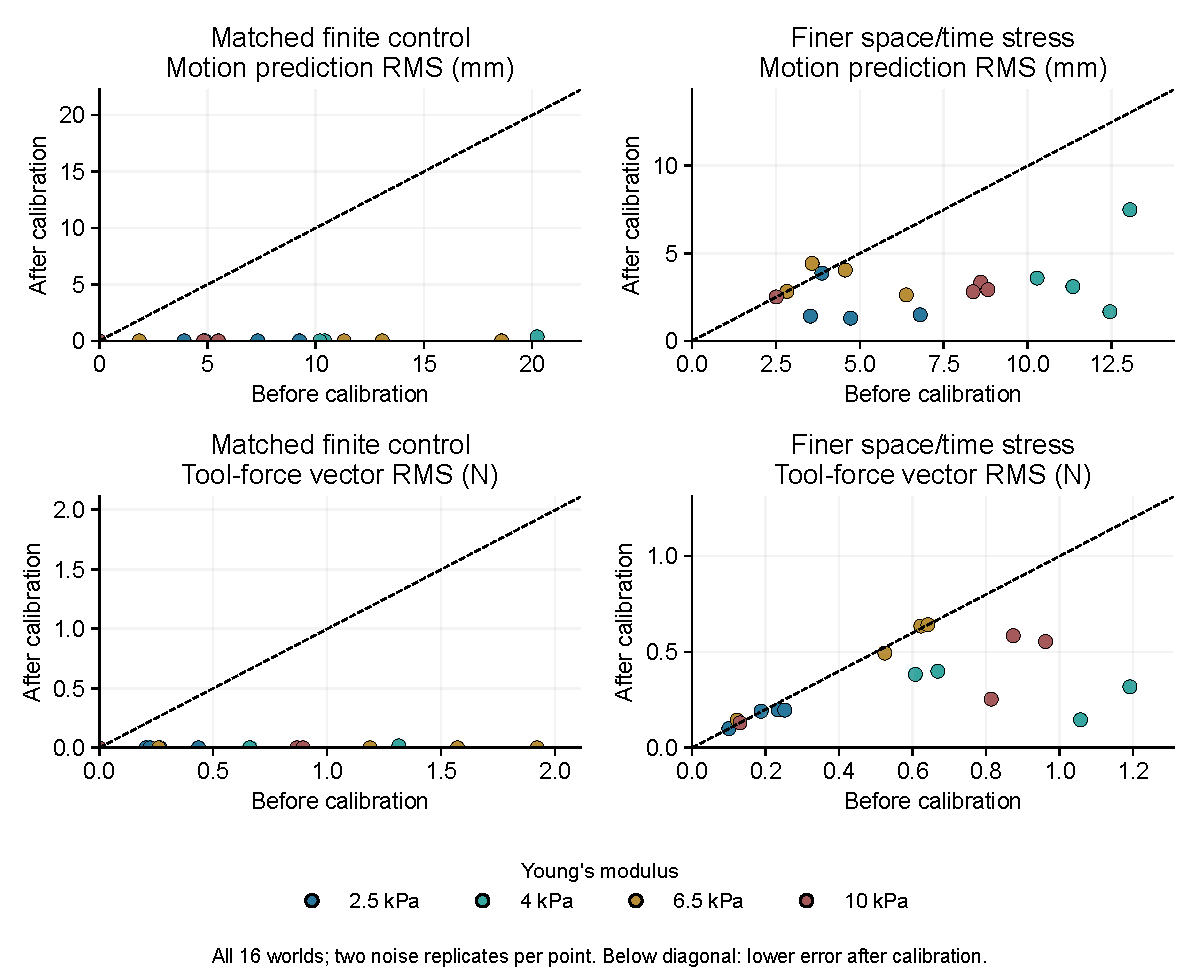
\includegraphics[width=.82\textwidth]{../../output/gap-first-v01/bowl/bowl-all-worlds.pdf}
\caption{All 16 parameter worlds in the controlled finite grid, not 16 distinct
objects. Each point averages two observation-noise replicates. Horizontal and
vertical axes give errors before and after selected calibration; points below
the diagonal improve. Colors identify Young's modulus, with four friction values
per modulus. The matched control and finer space/time stress are shown separately;
these plots do not establish superiority over the best fixed calibration action.}
\label{fig:bowl-all-worlds}
\end{figure*}
\begin{figure*}[t]
\centering
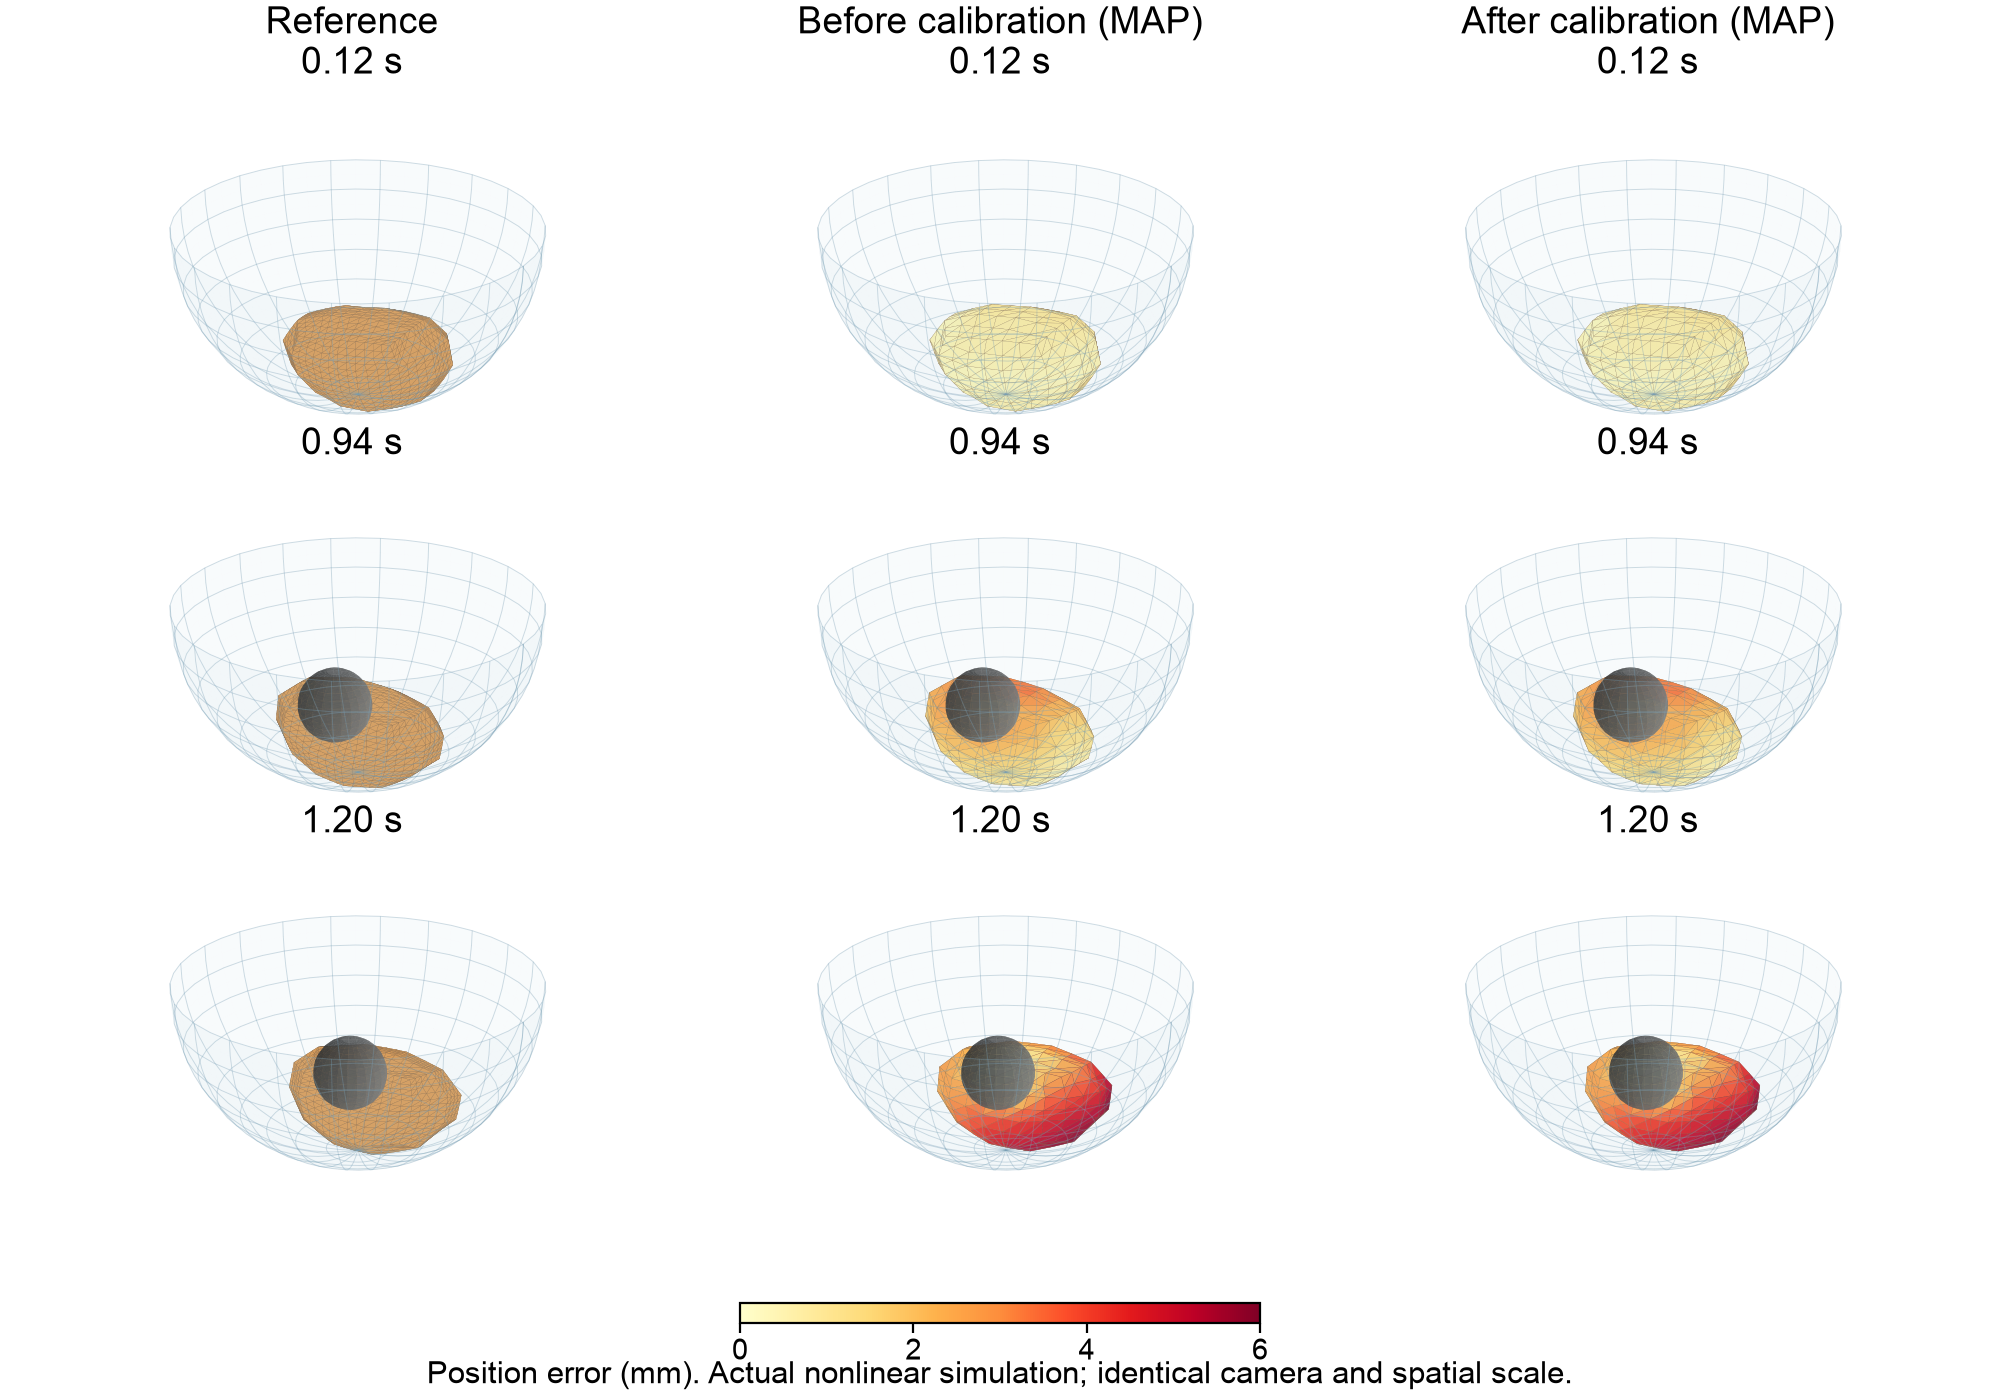
\includegraphics[width=.75\textwidth]{../../output/gap-first-v01/bowl/bowl-refined-case00.png}
\caption{Fixed world 0, noise replicate 0: actual finer-reference geometry and
coarse-only MAP predictions before/after calibration on a separate reset interaction.
All panels use the same camera and true spatial scale; no deformation amplification.
Color encodes position error and saturates at 6\,mm. This is simulated surface
geometry, not a photorealistic-rendering benchmark.}
\label{fig:bowl-fixed-case}
\end{figure*}
\begin{figure*}[t]
\centering
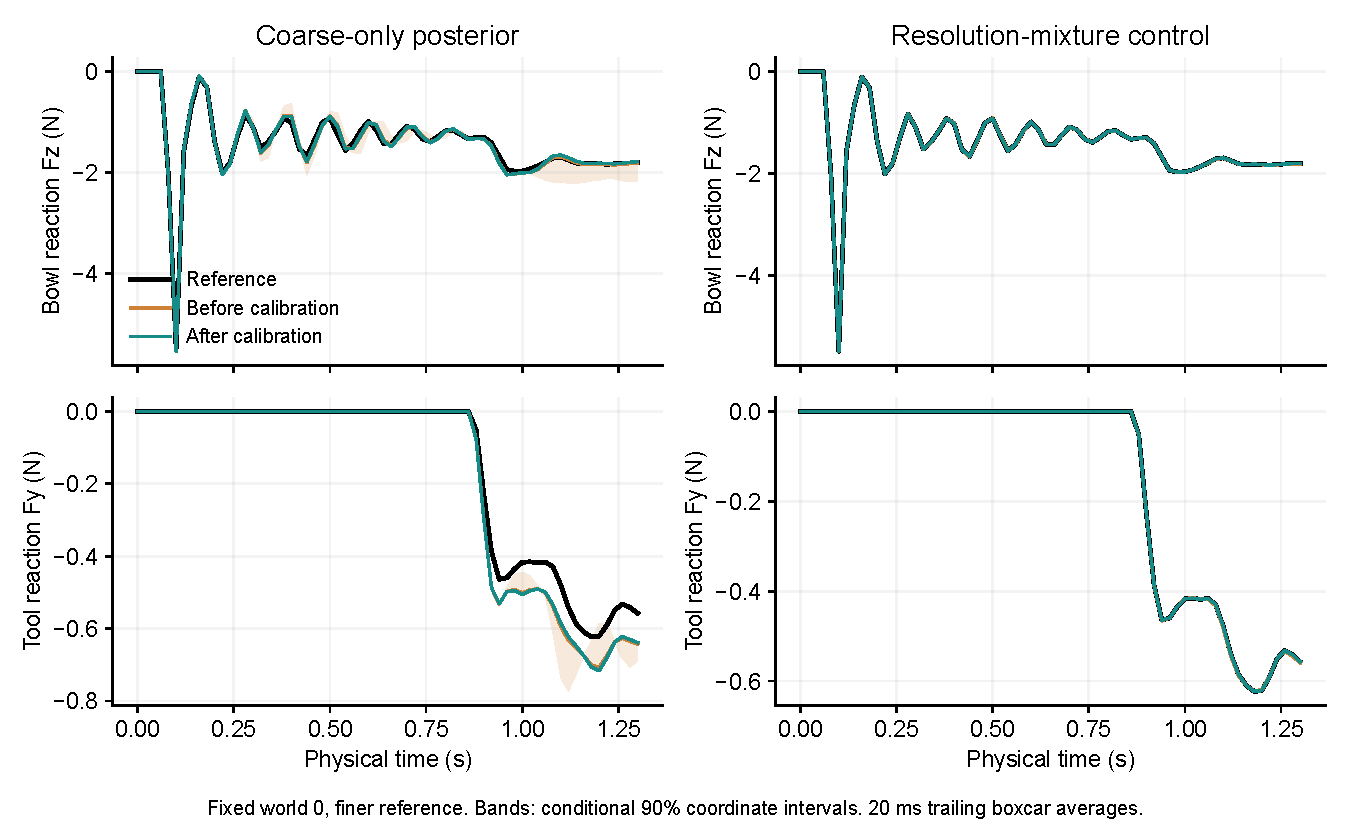
\includegraphics[width=.75\textwidth]{../../output/gap-first-v01/bowl/bowl-force-predictions.pdf}
\caption{Withheld reaction predictions for fixed world 0 of the finer-reference
stress. Only position tracks are observed. Shading gives conditional 90\% coordinate
intervals; the secondary resolution mixture contains the reference by construction.}
\label{fig:bowl-forces}
\end{figure*}
\paragraph{Observation and prediction protocol.}
Sixteen parameter worlds combine four moduli (2.5,4,6.5,10\,kPa) and four friction
coefficients (0.1,0.25,0.45,0.7). We supply four known surface correspondences
projected into an overhead camera, with 0.5\,mm independent coordinate noise.
Initial observations occur at 0.08 and 0.12\,s. Exactly one reset calibration
experiment is selected: a 25\,mm position-controlled push or a 0.2\,rad bowl rotation.
The latter moves the wall tangentially about a fixed spherical center; gravity
does not rotate. New coordinates at 0.94 and 1.2\,s update the posterior. The
separate held-out experiment applies a stronger 45\,mm transverse push after
entering through the open rim. No reaction-force measurements enter inference.

The primary risk is the posterior probability that the deployed MAP model
exceeds 3\,mm point RMS across 64 common material nodes at 1.1,1.2 and 1.3\,s.
This is a fixed-budget calibration comparison, not a proceed-or-acquire policy.
Both fixed actions and the same-evidence MAP predictor are controls. All action
choices and risks are sealed before scoring the selected-world held-out targets.
We evaluate 16 worlds at two discretizations, with two noise replicates each:
64 records, not 64 independent objects. Intervals resample the 16 world clusters.

\paragraph{Qualification and limits.}
Inference uses a 6-cell-per-axis mesh at 25\,$\mu$s; the finer space/time reference
uses 12 cells at 12.5\,$\mu$s, preserving the same piecewise-linear rest geometry.
A 12-cell 25\,$\mu$s development run failed the positive-volume check and is retained
as a numerical failure. The smaller-step soft/stiff controls complete with minimum
Jacobians 0.271/0.372 and sampled penetration 0.172/0.268\,mm. Dense saved-surface
penetration is audited separately. Halving the inference timestep changes the
development target by 0.35\,mm; changing both space and time resolution changes it
by 1.42 and 2.81\,mm. The latter is close to the 3\,mm decision tolerance: this is an
intentional numerical-model stress test, not converged continuum truth.
The open bowl has no rim thickness, continuous collision detection or self-contact.
All 1280 declared marker observations pass the surface/tool/bowl occlusion audit.

\paragraph{Conditional prediction and numerical-model uncertainty.}
Table~\ref{tab:bowl-gap-results} reports the predeclared primary coarse-only posterior
and a secondary 32-hypothesis resolution mixture. The mixture assigns prior 0.5 to
each resolution and the same uniform parameter prior within each. The finer
reference is therefore included by construction; this comparator demonstrates
conditional numerical-model uncertainty, not coverage of arbitrary unknown physics.
The complete report also compares both fixed actions and gives the mixture exactly
the coarse policy's chosen observation, separating model uncertainty from action
selection. Reaction-force errors use 20\,ms trailing boxcar averages accumulated
from every integration step, with bowl and tool scored separately in newtons.

\paragraph{Measured benefit and failure.}
In the matched finite control, selected calibration reduces mean MAP motion error
from 7.588 to 0.023\,mm, but fixed bowl rotation achieves zero MAP error; this does
not establish an advantage over the best fixed experiment. Against the finer
space/time reference, calibration reduces mean error from 6.981 to 3.091\,mm,
while 43.75\% of predictions exceed the 3\,mm tolerance despite a mean predicted
failure probability of only 1.856\%. Conditional 90\% coordinate intervals cover
only 6.14\% of reference coordinates. Fixed rotation has a lower 31.25\% failure
rate. Thus improved motion accuracy does not imply trustworthy uncertainty under
model mismatch. Given exactly the coarse policy's correction observations, the
resolution-mixture control reaches 0.051\,mm mean error and no failures, conditional
on the fine model being included by construction.









An unchanged PhysTwin spring-force kernel was also attempted under the shared
contact/integration adapter. It failed that adapter's positive-tetrahedron-volume
qualification across CPU/GPU and timestep checks. We retain the failure record but
exclude it from accuracy rankings; it is not evidence that the full native PhysTwin
method fails on bowls.


\clearpage
\balance
\section{What this establishes}
The useful distinction is between \emph{uncertain parameters}, \emph{uncertain task response}, and \emph{model inadequacy}. A wide material posterior can permit a safe repeated action. Another view can resolve a support/material tradeoff when informative geometry is visible. A calibrated interaction can distinguish explanations that the permitted cameras cannot separate. None of these statements makes uncertainty automatically trustworthy when contact, constitutive behavior or observation noise is misspecified.

The new experiments add a prediction-specific risk decision to the prior joint-field work, preserving its analytical marginalization where the observation model is linear Gaussian. They do not extend exact Gaussian force elimination to nonlinear impacts, establish arbitrary contact discovery, or claim that a finite set of physical hypotheses covers every real object. Likewise, a failed adapter qualification is not evidence that its source method fails natively. These distinctions keep the next step concrete: validate the observation model and hypothesis family, then assess whether the selected corrective evidence improves a different held-out interaction.

\paragraph{Artifacts and reproducibility.}
The campaign namespaces are \texttt{scripts/gap\_first\_v01}, \texttt{reports/gap-first-v01} and \texttt{output/gap-first-v01}. They contain frozen protocols, pre-outcome predictions, complete cohort outcomes, numerical qualifications, independent audits and actual-versus-predicted videos. Large released datasets and checkpoints remain local. This addendum supplements the existing manuscript and preserves its previously published experiments.

\begin{thebibliography}{9}
\bibitem{reconphys} Boyuan Wang et al. ReconPhys: Reconstruct Appearance and Physical Attributes from Single Video. arXiv:2604.07882, 2026. \url{https://arxiv.org/abs/2604.07882}.
\bibitem{gaussianbench} Chukwudalu Dumebi-Kachikwu. GaussianBench: Physics-Fidelity Evaluation for Gaussian Scene Representations. arXiv:2610.10554, 2026. \url{https://arxiv.org/abs/2610.10554}.
\bibitem{phystwin} Hanxiao Jiang, Hao-Yu Hsu, Kaifeng Zhang, Hsin-Ni Yu, Shenlong Wang, and Yunzhu Li. PhysTwin: Physics-Informed Reconstruction and Simulation of Deformable Objects from Videos. ICCV, 2025.
\end{thebibliography}
\end{document}
